\documentclass{report}
\usepackage{amsmath}
\usepackage{amsfonts}
\usepackage{graphicx}
\usepackage{listings}
\usepackage{hyperref}
\usepackage{pdfpages}

\renewcommand{\bibname}{References}

\title{Handwritten Digit Recognition on FPGA}
\date{}

\begin{document}
%
\includepdf[pages=1]{CoverPage.pdf}

\maketitle

\tableofcontents

\chapter{Introduction}
\section{Neural Network}
A neural network is a method in artificial intelligence that teaches computers to process data in a way that is inspired by the human brain. It is a type of machine learning process, called deep learning, that uses interconnected nodes or neurons in a layered structure that resembles the human brain. It creates an adaptive system that computers use to learn from their mistakes and improve continuously. Thus, artificial neural networks attempt to solve complicated problems, like summarizing documents or recognizing faces, with greater accuracy\cite{aws_nn}.

\subsection{Neural Network - Example}
Figure \ref{fig:NeuralNetwork} shows a simple neural network which has one input, one hidden and one output layer. Input and output layers contain two neurons each while hidden layer contain 3 neurons.
\begin{figure}[h!]
    \centering
    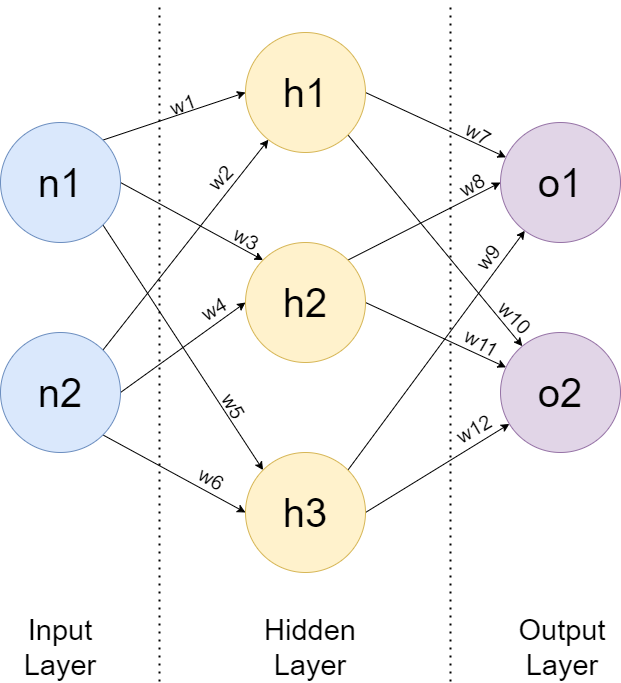
\includegraphics[width=0.5\textwidth]{NeuralNetwork.png}
    \caption{Neural Network Example}
    \label{fig:NeuralNetwork}
\end{figure}

\section{Why neural networks?}
Neural networks can help computers make intelligent decisions with limited human assistance. This is because they can learn and model the relationships between input and output data that are nonlinear and complex. They are widely used in making smart systems nowadays. 

\section{Field Programmable Gate Arrays (FPGAs)}
FPGAs are integrated circuits that can be configured by the user after manufacturing. They consist of an array of programmable logic blocks and a hierarchy of reconfigurable interconnects, allowing the creation of custom hardware circuits.

\section{Why FPGAs?}
Field Programmable Gate Arrays (FPGAs) offer several advantages for implementing neural networks:
\begin{itemize}
    \item \textbf{Parallelism:} FPGAs can exploit the inherent parallelism in neural network computations, allowing for concurrent execution of multiple operations. This leads to significant speedup compared to sequential processing on general-purpose processors.
    \item \textbf{Customization:} FPGAs can be customized to implement specific neural network architectures and operations, optimizing the hardware for the target application. This flexibility allows designers to balance performance, power consumption, and resource utilization.
    \item \textbf{Low Latency:} FPGAs provide deterministic and low-latency processing, which is critical for real-time applications such as autonomous driving, robotics, and financial trading.
    \item \textbf{Energy Efficiency:} FPGAs can be more energy-efficient than CPUs and GPUs for certain tasks, as they can be tailored to perform only the necessary computations with minimal overhead.
    \item \textbf{Reconfigurability:} FPGAs can be reconfigured to implement different neural network models or updated designs without changing the hardware. This reconfigurability makes FPGAs suitable for research and development environments where algorithms are constantly evolving.
\end{itemize}

\section{FPGA Design Workflow}
The workflow of an FPGA Based Design\cite{fpga_workflow} is given in the figure \ref{fig:fpga_workflow}.Figure \ref{fig:fpga_workflow} depicts a typical workflow for designing, verifying, and implementing a chip architecture. It begins with the "Concept" phase, where the idea and specifications for the chip are defined. This is followed by the "Design" phase, which includes developing the chip architecture and writing the hardware description language (HDL) code. The design is then subjected to "Verification" through simulation and testing to ensure it meets the specified requirements and functions correctly. If any issues are detected, the design is revised. Once verified, the design moves to the "Implementation" phase, where it undergoes synthesis to convert the HDL code into a gate-level netlist, and then place and route to arrange and connect the gates physically. This structured approach ensures that each step is thoroughly checked and corrected before progressing, thereby reducing errors and ensuring successful chip fabrication.
 
\begin{figure}[h!]
    \centering
    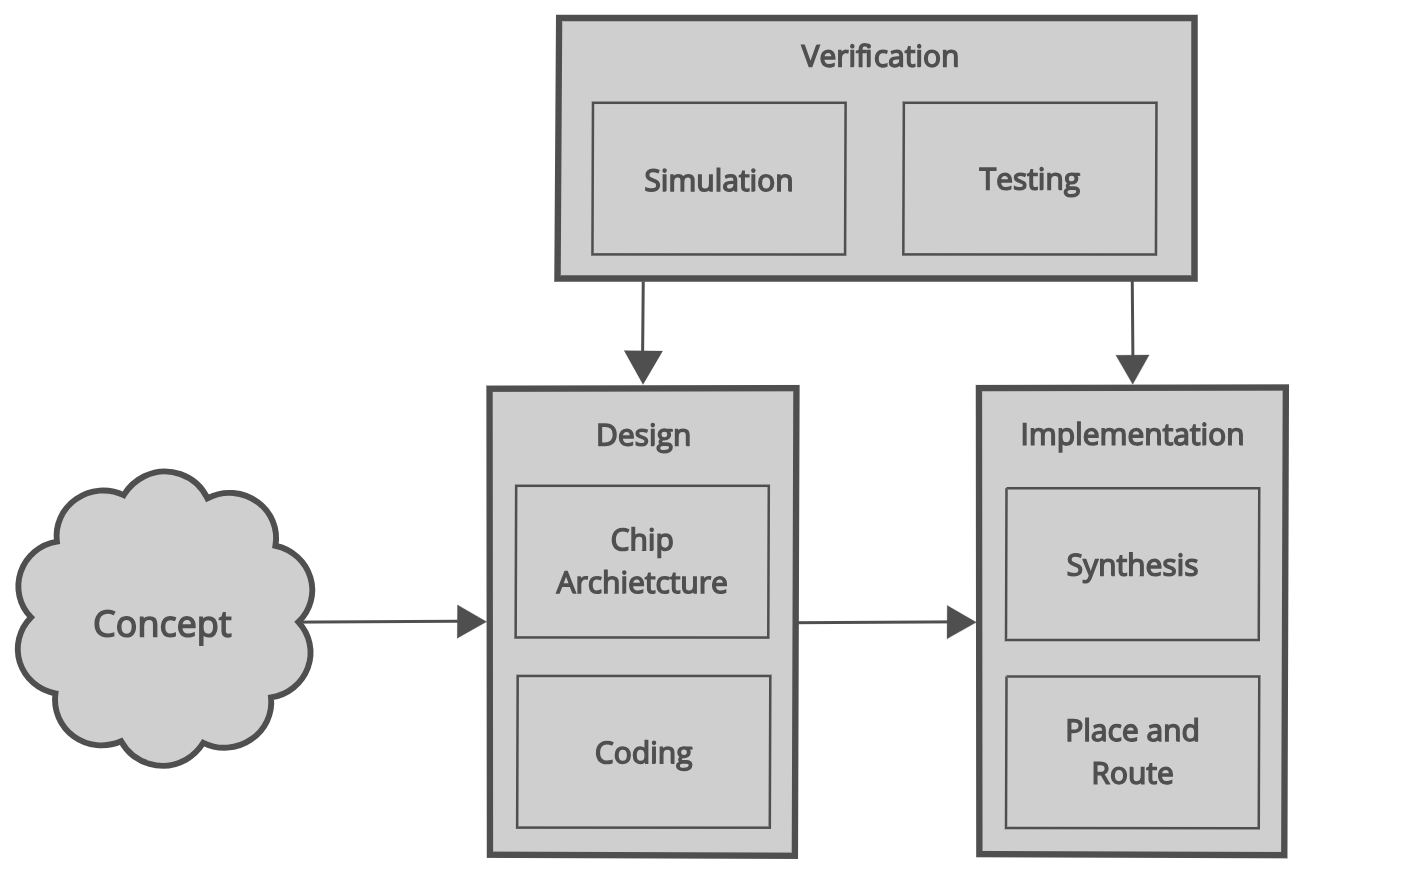
\includegraphics[width=0.6\textwidth]{fpga_workflow.png}
    \caption{FPGA Based Design Workflow}
    \label{fig:fpga_workflow}
\end{figure}

\section{Coding in FPGA}
Coding for FPGAs (Field Programmable Gate Arrays) involves writing hardware description language (HDL) code to define the behavior and structure of digital circuits. The two most commonly used HDLs are VHDL (VHSIC Hardware Description Language) and Verilog. Coding in FPGA involves several key considerations and steps to ensure efficient and functional hardware design. Coding for FPGAs requires a deep understanding of both hardware and software principles. Efficient FPGA coding can lead to highly optimized designs that exploit the parallelism and reconfigurability of FPGAs, making them ideal for applications requiring high performance, low latency, and energy efficiency. Proper coding practices, thorough verification, and effective use of synthesis tools are essential to successful FPGA design.

\section{Hardware Synthesis in FPGA}
During the FPGA synthesis process\cite{fpga_synthesis}, a high description design or an HDL design is converted into a gate level representation or a logic component. This means that FPGA code provided in high level language such as VHDL or Verilog is converted into logic gates using a synthesis tool as shown in figure \ref{fig:fpga_synthesis}.

\begin{figure}[h!]
    \centering
    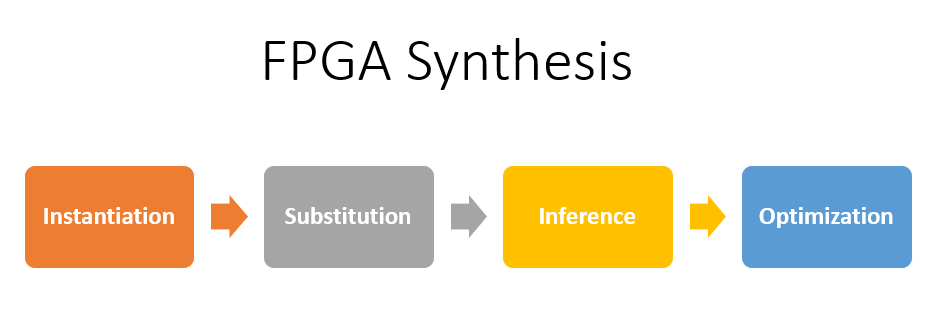
\includegraphics[width=0.75\textwidth]{fpga_synthesis.png}
    \caption{FPGA Synthesis Workflow}
    \label{fig:fpga_synthesis}
\end{figure}

\section{High-Level Synthesis (HLS)}
HLS is a method of transforming a high-level algorithmic description of a circuit into a register-transfer level (RTL) design. HLS tools can automatically generate hardware descriptions from C, C++, or SystemC code, significantly reducing the design time. Its general workflow can be seen in figure \ref{fig:hls_workflow}.

\begin{figure}[h!]
    \centering
    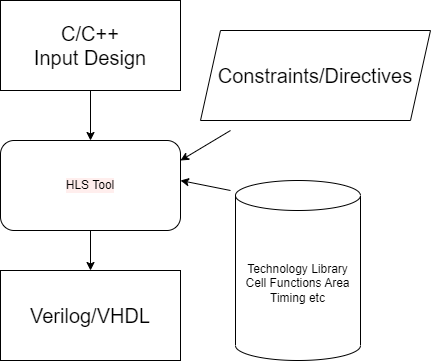
\includegraphics[width=0.6\textwidth]{hls_workflow.png}
    \caption{HLS Synthesis Workflow}
    \label{fig:hls_workflow}
\end{figure}

\section{FPGAs for Neural Networks}
FPGAs present a compelling option for neural network implementations due to their flexibility, performance, and efficiency. They are particularly suited for applications requiring real-time processing, low latency, and energy efficiency. With ongoing advancements in FPGA technology and development tools, their adoption in neural network applications is expected to grow, bridging the gap between general-purpose processors and dedicated hardware accelerators.

\chapter{Neural Network Implementation - Making a Model}

\section{Model Training}
First step is to train a machine learning model using tools like Jupyter Notebook, Google Colab etc. In this project, we have used Google Colab for training a tensor flow model for handwritten digit recognition as shown in figure \ref{fig:training_model1}.


\begin{figure}[h!]
    \centering
    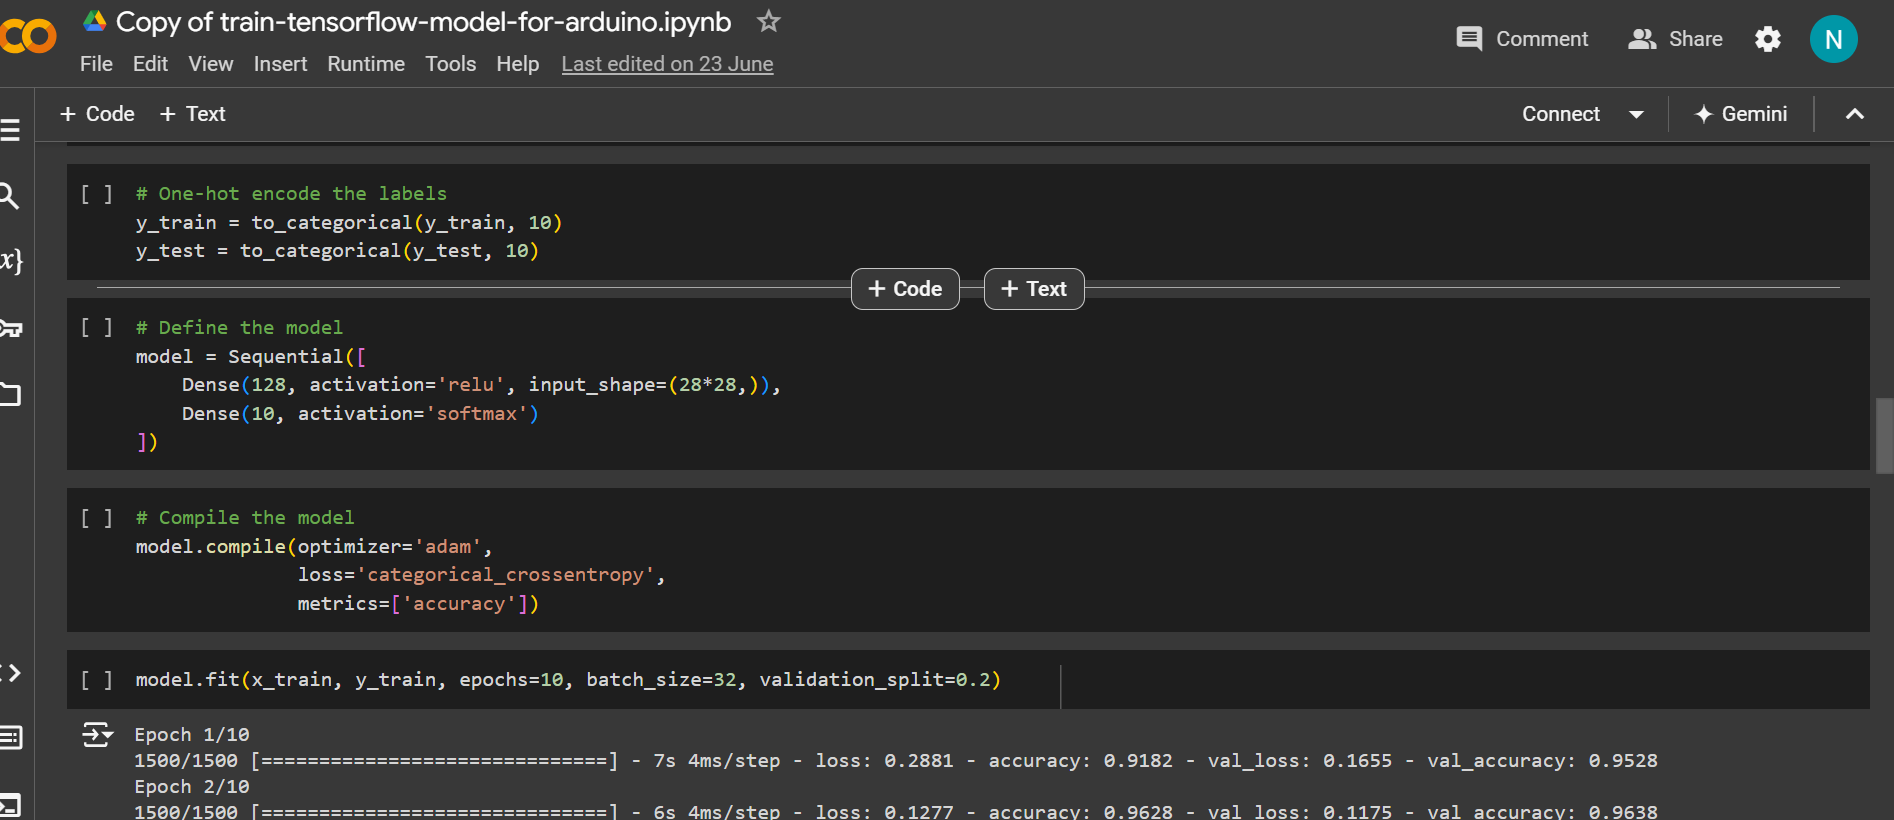
\includegraphics[width=\textwidth]{training_model2.png}
    \caption{Model Training in Google Colab}
    \label{fig:training_model1}
\end{figure}

\subsection{Training Data}
For training, we have used MNIST dataset. The MNIST (Modified National Institute of Standards and Technology) dataset is a benchmark dataset widely used in the field of machine learning and computer vision, specifically for handwritten digit recognition. It consists of images of handwritten digits from 0 to 9 and serves as a standard for evaluating and comparing the performance of various algorithms and models.
It consist of images as shown in figure \ref{fig:mnist}.

\begin{figure}[h!]
    \centering
    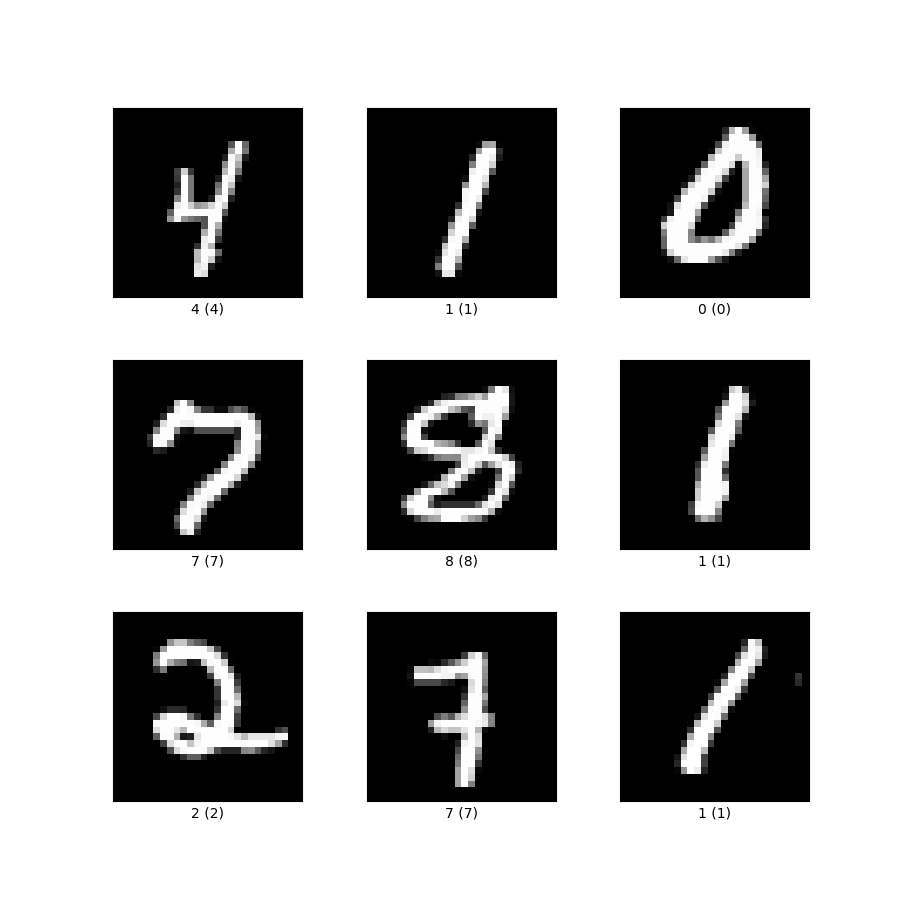
\includegraphics[width=\textwidth]{mnist.png}
    \caption{MNIST Dataset Sample}
    \label{fig:mnist}
\end{figure}

\section{Structure of Model}
The model consists of two dense (fully connected) layers. The first layer has 128 hidden units, and the second layer has 10 output units corresponding to 10 possible classes. The network architecture is as follows:

\begin{itemize}
    \item Input layer: 784 units (28x28 pixels)
    \item Dense layer 1: 128 units
    \item ReLU activation
    \item Dense layer 2: 10 units
    \item Softmax activation
\end{itemize}

\section{Extraction of weights and biases from the network}
Using the below Python Code, We succesfully extracted the weights and biases from the trained model. These weights and biases were then used in Vivado HLS\cite{vivado_hls} C++ code. 

\begin{lstlisting}[language=Python]
# Save the trained model weights and biases
hidden_weights, hidden_biases = model.layers[1].get_weights()
output_weights, output_biases = model.layers[2].get_weights()

# Save the weights and biases to a file
np.savez('mnist_weights_biases.npz', 
         hidden_weights=hidden_weights, 
         hidden_biases=hidden_biases, 
         output_weights=output_weights, 
         output_biases=output_biases)
\end{lstlisting}

\chapter{Neural Network Implementation - High Level Implementation in Vivado HLS}

\section{Functions Implementations}
Following sections shows the code for implementation of the functions present in the model.

\subsection{Exponential Approximation}
We begin with the exponential function. The exponential function is approximated using a truncated Taylor series for computational efficiency:

\begin{lstlisting}[language=C++]
data_t exp_approx(data_t x) {
    const int num_terms = 10;
    data_t result = 1.0;
    data_t term = 1.0;

    for (int i = 1; i < num_terms; ++i) {
        term *= x / i;
        result += term;
    }
    return result;
}
\end{lstlisting}

\subsection{ReLU Activation}
The ReLU activation function is applied element-wise to the output of the first dense layer:

\begin{lstlisting}[language=C++]
void relu(data_t input[HIDDEN_SIZE], data_t output[HIDDEN_SIZE]) {
    for (int i = 0; i < HIDDEN_SIZE; i++) {
        output[i] = input[i] > 0 ? input[i] : 0;
    }
}
\end{lstlisting}

\subsection{Softmax Activation}
The softmax function normalizes the output of the second dense layer to a probability distribution:

\begin{lstlisting}[language=C++]
void softmax(data_t input[OUTPUT_SIZE], data_t output[OUTPUT_SIZE]) {
    data_t max_val = input[0];
    for (int i = 1; i < OUTPUT_SIZE; i++) {
        if (input[i] > max_val) {
            max_val = input[i];
        }
    }

    data_t sum = 0;
    for (int i = 0; i < OUTPUT_SIZE; i++) {
        output[i] = exp_approx(input[i] - max_val);
        sum += output[i];
    }

    for (int i = 0; i < OUTPUT_SIZE; i++) {
        output[i] /= sum;
    }
}
\end{lstlisting}

\section{Layers Implementations}
Following sections shows the code for implementation of the layers present in the model.

\subsection{Dense Layers}
The dense layers are implemented as follows:

\begin{lstlisting}[language=C++]
void dense_1(data_t input[INPUT_SIZE], data_t output[HIDDEN_SIZE], 
const data_t weights[INPUT_SIZE][HIDDEN_SIZE], const data_t bias[HIDDEN_SIZE]) {
    for (int i = 0; i < HIDDEN_SIZE; i++) {
        data_t sum = bias[i];
        for (int j = 0; j < INPUT_SIZE; j++) {
            sum += input[j] * weights[i][j];
        }
        output[i] = sum;
    }
}

void dense_2(data_t input[HIDDEN_SIZE], data_t output[OUTPUT_SIZE], 
const data_t weights[HIDDEN_SIZE][OUTPUT_SIZE], const data_t bias[OUTPUT_SIZE]) {
    for (int i = 0; i < OUTPUT_SIZE; i++) {
        data_t sum = bias[i];
        for (int j = 0; j < HIDDEN_SIZE; j++) {
            sum += input[j] * weights[i][j];
        }
        output[i] = sum;
    }
}
\end{lstlisting}

\section{Top-level Function}
The top-level function integrates the layers and activation functions:

\begin{lstlisting}[language=C++]
void neural_network(data_t input[INPUT_SIZE], data_t output[OUTPUT_SIZE],
                    const data_t dense_1_weights[INPUT_SIZE][HIDDEN_SIZE], 
										const data_t dense_1_bias[HIDDEN_SIZE],
                    const data_t dense_2_weights[HIDDEN_SIZE][OUTPUT_SIZE], 
										const data_t dense_2_bias[OUTPUT_SIZE]) {

    #pragma HLS INTERFACE m_axi port=input offset=slave bundle=gmem
    #pragma HLS INTERFACE m_axi port=output offset=slave bundle=gmem
    #pragma HLS INTERFACE m_axi port=dense_1_weights offset=slave bundle=gmem
    #pragma HLS INTERFACE m_axi port=dense_1_bias offset=slave bundle=gmem
    #pragma HLS INTERFACE m_axi port=dense_2_weights offset=slave bundle=gmem
    #pragma HLS INTERFACE m_axi port=dense_2_bias offset=slave bundle=gmem
    #pragma HLS INTERFACE s_axilite port=return bundle=control

    data_t dense_1_out[HIDDEN_SIZE];
    data_t relu_out[HIDDEN_SIZE];
    data_t dense_2_out[OUTPUT_SIZE];

    // Layer 1: Dense
    dense_1(input, dense_1_out, dense_1_weights, dense_1_bias);

    // Layer 1: ReLU Activation
    relu(dense_1_out, relu_out);

    // Layer 2: Dense
    dense_2(relu_out, dense_2_out, dense_2_weights, dense_2_bias);

    // Layer 2: Softmax Activation
    softmax(dense_2_out, output);
}
\end{lstlisting}

\chapter{Testing and Verification}
This chapter describes the testing of the neural network on the FPGA. In this phase,  we write a testbench code for testing the design under test which is our neural network for recognizing handwritten digits.

\section{Testbench}
Below is the code for testbench for our project design.

\begin{lstlisting}[language=C++]
#include <iostream>
#include <cmath>
#include "mnist_image_array.h"

#define INPUT_SIZE 784  // 28 * 28
#define HIDDEN_SIZE 128
#define OUTPUT_SIZE 10

typedef float data_t;

// Function prototypes
void neural_network(data_t input[INPUT_SIZE], data_t output[OUTPUT_SIZE],
                    const data_t dense_1_weights[INPUT_SIZE][HIDDEN_SIZE], const data_t dense_1_bias[HIDDEN_SIZE],
                    const data_t dense_2_weights[HIDDEN_SIZE][OUTPUT_SIZE], const data_t dense_2_bias[OUTPUT_SIZE]);

// Helper function to print the output array
void print_output(data_t output[OUTPUT_SIZE]) {
    float max = 0;
    int index, i;
	for ( i = 0; i < OUTPUT_SIZE; i++) {
        if(output[i] > max){
        	max = output[i];
        	index = i;
        }
      	std::cout << "Output[" << i << "] = " << output[i] << std::endl;
    }
	std::cout << "Predicted Number = "<< index <<" with P = "<< max << std::endl;
}

int main() {
    // Declare and initialize input data in .h

	// Declare and initialize output array
    data_t output[OUTPUT_SIZE];

    // Declare and initialize dense_1_weights and dense_1_bias
    const data_t dense_1_weights[INPUT_SIZE][HIDDEN_SIZE] = {..};
    const data_t dense_1_bias[HIDDEN_SIZE] = {..};

    // Declare and initialize dense_2_weights and dense_2_bias
    const data_t dense_2_weights[HIDDEN_SIZE][OUTPUT_SIZE] = {..};

    const data_t dense_2_bias[OUTPUT_SIZE] = {...};

    // Call the neural network function
    neural_network(image, output, dense_1_weights, dense_1_bias, dense_2_weights, dense_2_bias);

    // Print the output
    print_output(output);

    return 0;
}

}
\end{lstlisting}


\section{Breakdown of testbench code}
Here is a brief summary of the testbench code, we wrote for testing the project design.

\begin{itemize}
    \item The \texttt{main} function starts by declaring and initializing the input data, output array, and weights and biases for both dense layers.
    \item The input data is assumed to be declared and initialized in the included header file.
    \item The weights and biases are initialized to empty arrays here to save space.
    \item The \texttt{neural\_network} function is called with the input image and weight/bias parameters.
    \item The output of the neural network is then printed using the \texttt{print\_output} function.
\end{itemize}


\section{Inputting Image to Model}
Using a Python script, we were able to convert a 28x28 image to a 784 elements, one dimensional array. 

\begin{lstlisting}[language=Python]
from PIL import Image
import numpy as np

# Function to process image and save as C array
def image_to_c_array(image_path, output_path):
    # Open the image file
    img = Image.open(image_path).convert('L')  # Convert to grayscale

    # Resize image to 28x28 if it's not already
    img = img.resize((28, 28))

    # Convert image to numpy array and normalize pixel values
    img_array = np.array(img) / 255.0

    # Flatten the array
    flat_array = img_array.flatten()

    # Convert to C array format
    c_array_str = ', '.join(map(str, flat_array))
    c_array = f"float image[784] = {{ {c_array_str} }};"

    # Write to output file
    with open(output_path, 'w') as file:
        file.write(c_array)

    print(f"C array saved to {output_path}")

\end{lstlisting}

\chapter{Results}

The performance and accuracy of the implemented neural network are evaluated. This chapter includes the testing methodology, performance metrics, and comparison with other implementations.

\section{Performance Metrics}
The performance of the network is measured in terms of latency, throughput, and resource utilization on the FPGA. The results are summarized in the following figure \ref{fig:utilization_estimates}. By doing some approximations, we were able to decrease the LUT utilization to almost 50\%. We changed the datatype from float to 16 bit ap\_fixed in which only 8 bits were reserved for the floating point and rest 8 for the integer part.


\begin{figure}[h!]
    \centering
    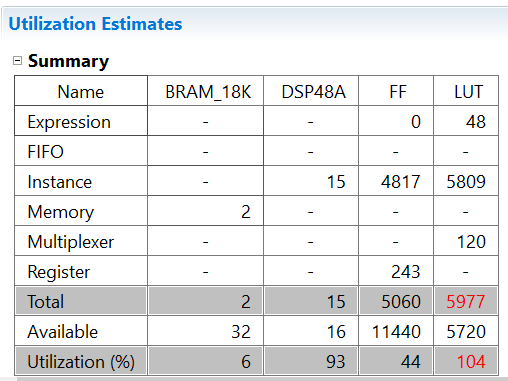
\includegraphics[width=0.75\textwidth]{utilization_estimates.png}
    \caption{Summary of the Utilization Estimates of the Project Design}
    \label{fig:utilization_estimates}
\end{figure}


\section{Output of Testbench in Vivado HLS}
Figure \ref{fig:output_4} shows the output of project design in Vivado HLS for the input image shown in \ref{fig:mnist_4}.

\begin{figure}[h!]
    \centering
    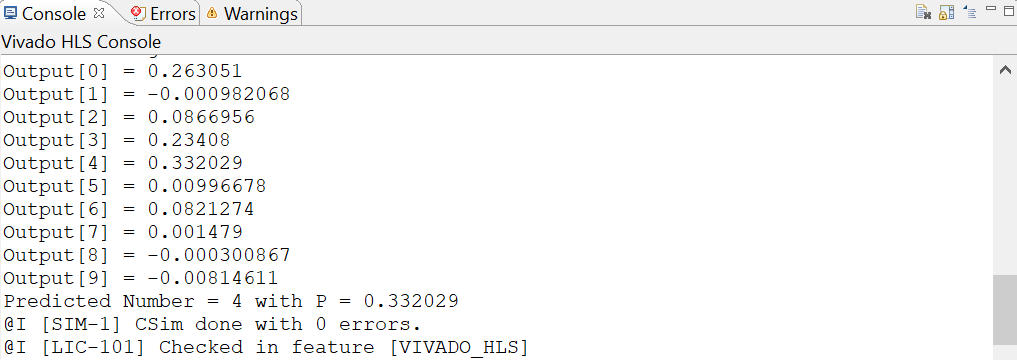
\includegraphics[width=\textwidth]{output_4.png}
    \caption{Output for Handwritten Image of 4}
    \label{fig:output_4}
\end{figure}

\begin{figure}[h!]
    \centering
    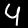
\includegraphics[width=28]{mnist_4.png}
    \caption{Input Image for 4}
    \label{fig:mnist_4}
\end{figure}

\chapter{Conclusion}
This report demonstrated the implementation of a neural network on an FPGA using HLS. The design achieved efficient performance by leveraging hardware parallelism and custom approximations for mathematical functions. Future work includes optimizing the design further and extending it to more complex networks. We can export the generated RTL to ISE using the Export RTL in Vivado HLS.In this way, we can implement this neural network on FPGA hardware.


\begin{thebibliography}{9}

\bibitem{aws_nn}
https://aws.amazon.com/what-is/neural-network

\bibitem{fpga_workflow}
https://fpgatutorial.com/introduction-to-fpga-development/

\bibitem{fpga_synthesis}
https://hardwarebee.com/understanding-fpga-logic-synthesis/

\bibitem{vivado_hls}
https://www.xilinx.com/products/design-tools/vivado/high-level-design.html
\end{thebibliography}

\end{document}
